\documentclass[UTF8]{ctexart}
\usepackage{hyperref}
\usepackage{abstract}
\usepackage[margin=1in]{geometry}
\usepackage{graphicx}
\begin{document}

\title{弦振动实验}
\author{2019012137  物理92  张鸿琳}
\maketitle
\begin{abstract}

本实验目的是推导弦振动方程,即波动方程,验证其正确性,同时利用方程预测在不同临界条件下的现象,实验观察并验证。实验中首先通过对小段线在微小振动中的受力情况推导出了弦振动方程,根据方程,找到了波速与弦线参数:张力,线密度的关系,进而通过测量波速求得了不同情况下的线密度;之后分别在固定和释放末端的条件下,通过不同的边界条件,预测并证实了其现象;最后,通过方程,推导出在两个固定边界条件下,存在一种稳定的波——“驻波”,预测并证实了其存在的性质。通过这一系列实验,充分验证了波动方程的正确性以及其对现象解释的准确性。


\centering
\textbf{Keywords:}波动方程,临界条件,驻波
\end{abstract}

\newpage
\tableofcontents
\newpage
\section{数据处理}
\subsection{推导弦振动方程,观察脉冲在弦上的传播现象并测试其速度}
(本实验原始数据见“原始测量数据”表一)
通过对小段弦线的受力分析,可以得到,在小振动下,若弦线张力为T,线密度为$\rho$,则满足波动方程$\frac{\partial^2 y}{\partial t^2}-\frac{T}{\rho}\frac{\partial^2 y}{\partial x^2}=0$,其通解为$y=f(vt\pm x)$,其中v为波速,又等于$\sqrt{\frac{T}{\rho}}$,故而在已知张力的条件下,可以求得对应的线密度$\rho=\frac{T}{v^2}$,原始测量数据处理结果如下表:
\begin{table}[htbp!] 
\centering 
\begin{tabular}{|c|c|c|c|c|} 
\hline 
 张力T(N)&距离s(cm) &  传播时间t(s)&波速v(m/s)& 线密度$\rho$(kg/m)  \\ 
\hline 
 1&4.39&3.45&0.012725&6176.026  \\ 
\hline 
 2&3.50 &0.91&0.038462&1352\\ 
\hline 
 4&2.11&0.33&0.063939&978.4147 \\ 
\hline
\end{tabular} 
\end{table}

\subsection{观察并分析弦线末端固定或松动时脉冲的反射现象}
(本实验原始数据见“原始测量数据”表二)在边界处固定时,满足边界条件$y|_{x=L_0}=0$,进而得到此时$y^-=-y^+$。若边界处松动,竖直方向上不受力,故满足边界条件$\frac{\partial y}{\partial x}|_{L_0}=0$,进而得到$\frac{\partial y^-}{\partial x}|_{L_0}=-\frac{\partial y^+}{\partial x}|_{L_0}$,可知,在该条件下二者振幅相同,频率相等,而方向相反,故而在末端叠加的最大振幅为原振幅两倍,从测量数据可知,实际数据符合地很好。

\subsection{观测弦线在周期性激励下的受迫振动和共振(或驻波)现象}
(本实验原始数据见“原始测量数据”表三)在弦线上传播的波满足简谐波方程,$y=Asin(\omega t-kx)$,其传播速度为$v=\frac{\omega}{k}=f\lambda$,故在已知波长和频率$f=1.00Hz$的条件下,同样可以求得波速,对原始测量数据进行处理得到下表:
\begin{table}[htbp!] 
\centering 
\begin{tabular}{|c|c|c|} 
\hline 
张力T(N) &  波长$\lambda$(cm)&波速v(m/s)  \\ 
\hline 
1 & 1.21 &0.0121\\ 
\hline
2 & 3.75 &0.0375\\ 
\hline 
4 & 6.21 &0.0621 \\  
\hline
\end{tabular} 
\end{table}

与第一个实验测得波速符合的很好,验证了该公式的正确性。

在固定边界条件下,也就是说相当于波可在两个边界处不断反射,如果要保持稳定,则必须满足驻波条件,即$L_0=\frac{n\lambda}{2}$,此时满足的波动方程为$y=-2A_0sin(kx)cos(\omega t)$,每点都在各自位置上做振幅不同的简谐振动,且存在固定的稳定点,即“驻点”,又由$v=f\lambda$,可以得到驻波频率与弦线参数的关系为:$f_n=\frac{nv}{2L_0}=\frac{n}{2L_0}\sqrt{\frac{T}{\rho}}$,故而可以求得在张力最大时,n等于1到3时对应的驻波频率,根据这些数据,通过实验验证,确实形成了明显且稳定的驻波,在激励振幅较小的的情况下,可以近似认为两个边界皆为固定,由于不断输入能量,振幅不断增大,达到2cm时的波图像见于“原始测量数据”。其分别对应的频率见下表:
\begin{table}[htbp!] 
\centering 
\begin{tabular}{|c|c|c|} 
\hline 
n &  波速v(m/s)&驻波频率($Hz$)  \\ 
\hline 
1 &0.0621 &0.414 \\ 
\hline
2 &0.0621&0.828  \\ 
\hline 
3 &0.0621&1.242 \\  
\hline
\end{tabular} 
\end{table}

\section{讨论}
本实验对于一些常见的波动现象运用波动方程进行了探究,但是一些方面仍然不够全面,比如在第三个实验中的驻波部分,将频率锁定在满足驻波条件的频率下,仅仅观察驻波的特性,而没有关注不满足驻波条件的频率会引发怎样的波动形式,它们无法稳定存在的现象也值得观察和进一步探究,从而使得实验更加具有全面性和一般性;另外对于驻波振幅不断增大的过程没有定量描述,可以通过方程推导在整个过程中振幅随时间变化过程,使得这部分过程更加清晰。
\section{原始测量数据}
\subsection{“推导弦振动方程,观察脉冲在弦上的传播现象并测试其速度”的原始数据}
在第一个实验中,由网站模拟出了下列数据:
\begin{table}[htbp!] 
\centering 
\begin{tabular}{|c|c|c|} 
\hline 
 张力T(N)&距离s(cm) &  传播时间t(s) \\ 
\hline 
 1&4.39&3.45  \\ 
\hline 
 2&3.50 &0.91\\ 
\hline 
 4&2.11&0.33 \\ 
\hline
\end{tabular} 
\end{table}
\subsection{“观察并分析弦线末端固定或松动时脉冲的反射现象”的原始数据}
在第二个实验中,由网站模拟出了下列数据:
\begin{table}[htbp!] 
\centering 
\begin{tabular}{|c|c|} 
\hline 
类型 & 振幅(cm)  \\ 
\hline 
入射脉冲 & 1.11 \\ 
\hline
末端最大幅度 &2.22\\ 
\hline 
反射脉冲& 1.11  \\  
\hline
\end{tabular} 
\end{table}
\subsection{“观测弦线在周期性激励下的受迫振动和共振(或驻波)现象”的原始数据}
在第三个实验中,由网站模拟出了下列数据(在满足驻波频率的条件下,观测到的波如下图):
\begin{table}[htbp!] 
\centering 
\begin{tabular}{|c|c|} 
\hline 
张力T(N) &  波长$\lambda$(cm)  \\ 
\hline 
1 & 1.21 \\ 
\hline
2 & 3.75 \\ 
\hline 
4 & 6.21  \\  
\hline
\end{tabular} 
\end{table}
\begin{center} 
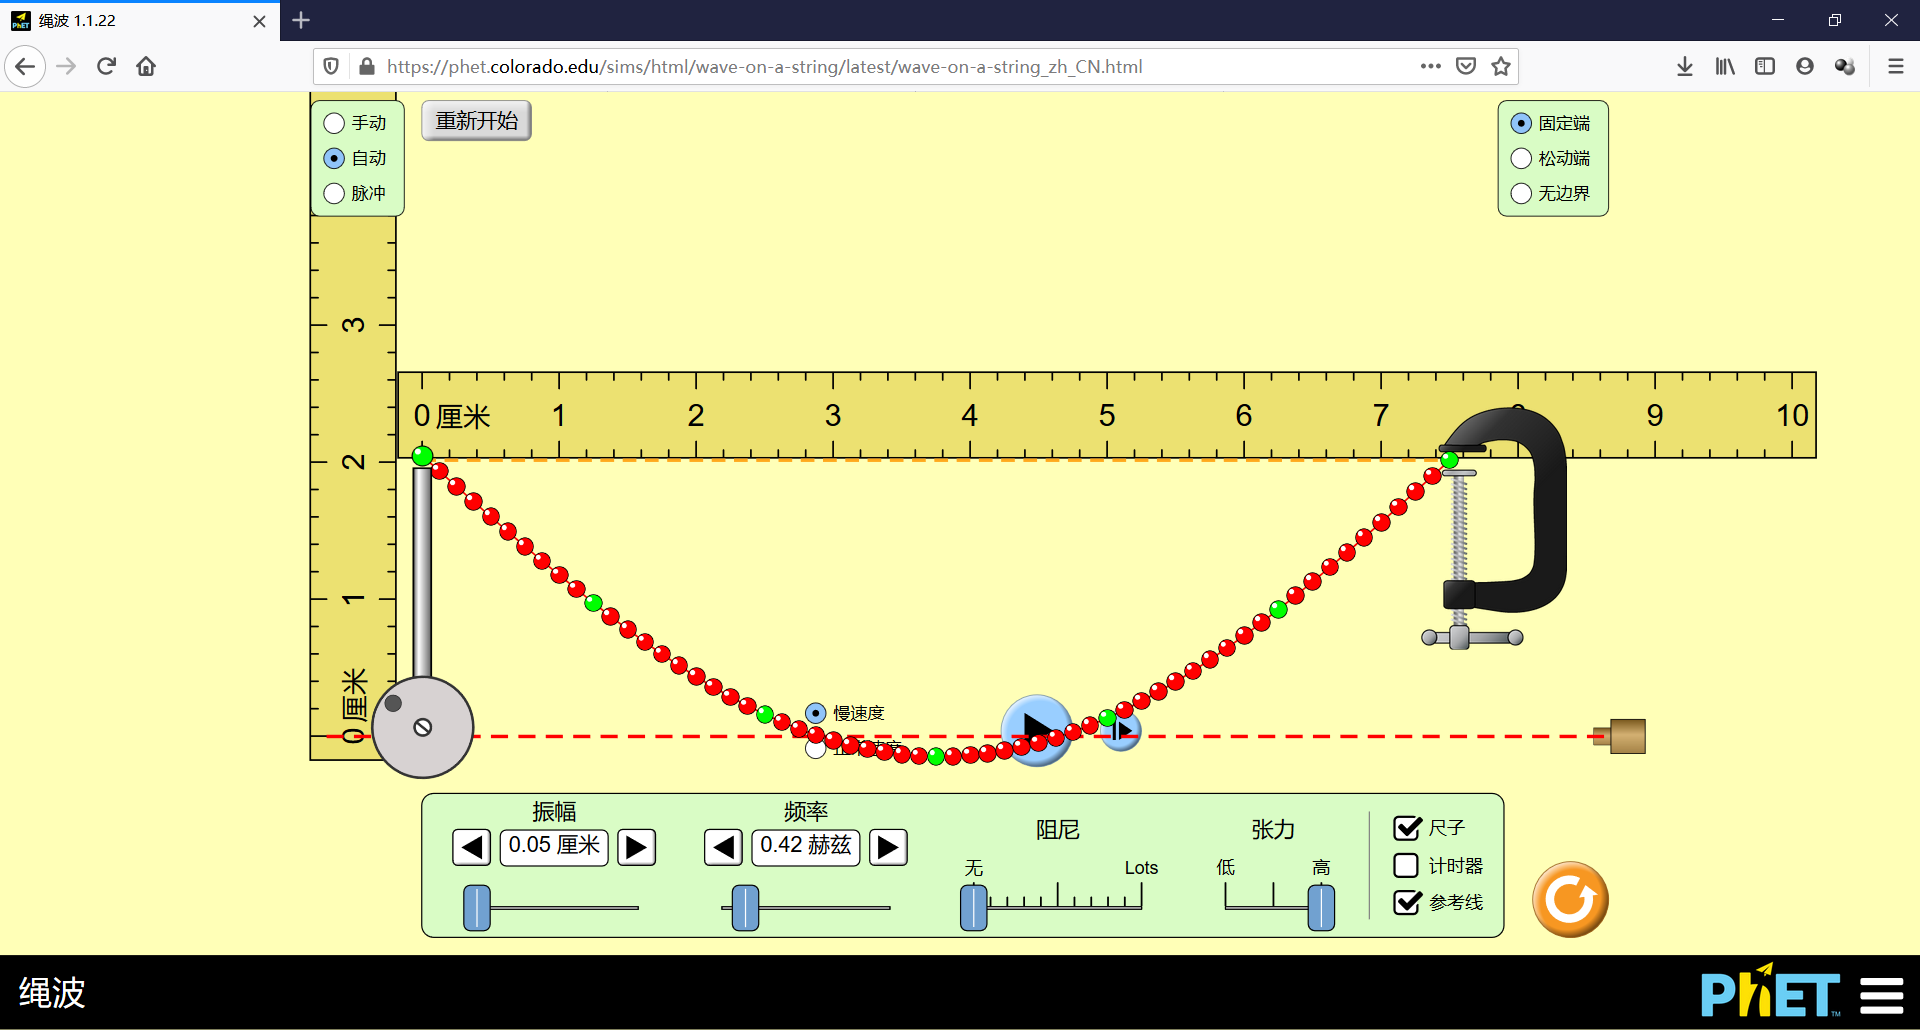
\includegraphics[width=0.95\textwidth]{A.png} 
\end{center}
\begin{center} 

\includegraphics[width=0.95\textwidth]{B.png} 
\end{center}
\begin{center} 
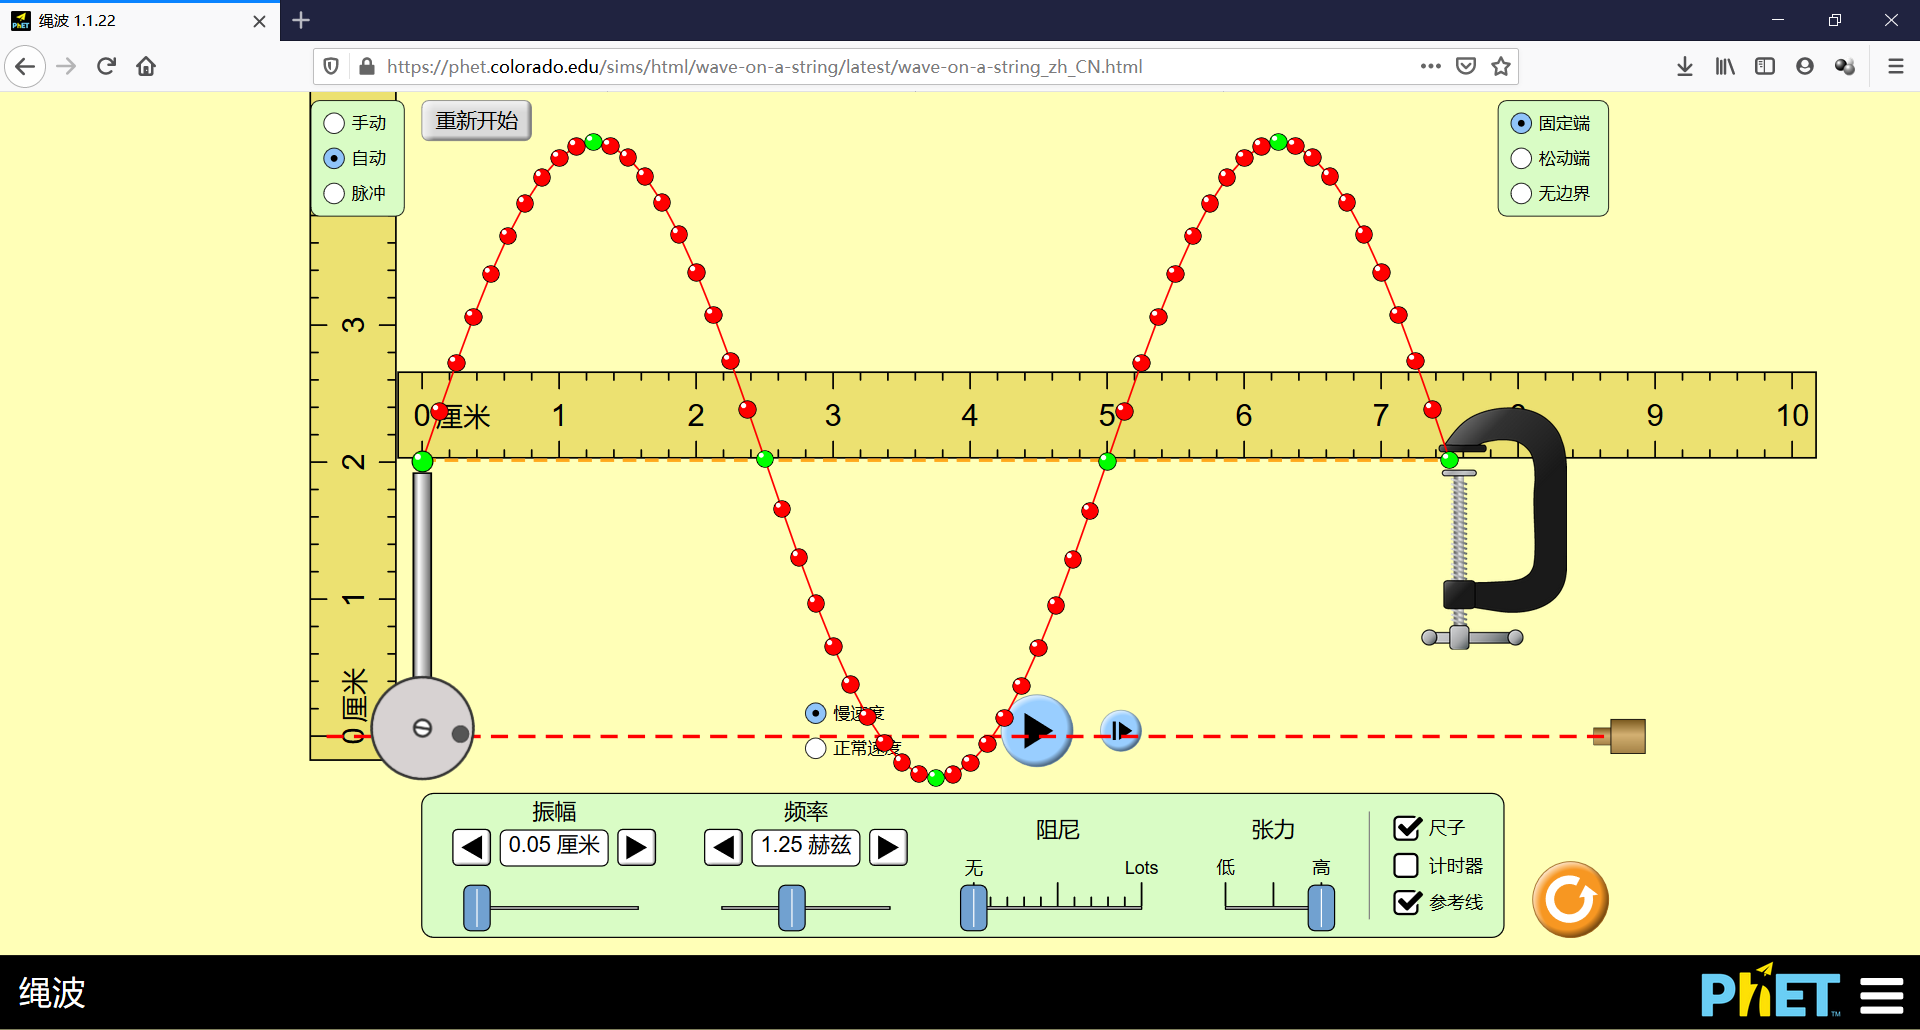
\includegraphics[width=0.95\textwidth]{C.png} 
\end{center}
\begin{thebibliography}{123456} 
\bibitem{ref1} 朱鹤年. 新概念基础物理实验讲义. 清华大学出版社. 2013. 
\bibitem{ref2} PhET:免费的在线物理、化学、生物、地理及数学仿真程序
\bibitem{ref3} 梁昆淼. 数学物理方法. 高等教育出版社. 1978.7.[图书馆有电子图书] 
\end{thebibliography}


\end{document}
